\documentclass{beamer}
\mode<presentation>
\usepackage{amsmath}
\usepackage{amssymb}
%\usepackage{advdate}
\usepackage{adjustbox}
\usepackage{subcaption}
\usepackage{enumitem}
\usepackage{multicol}
\usepackage{mathtools}
\usepackage{listings}
\usepackage{url}
\def\UrlBreaks{\do\/\do-}
\usetheme{Boadilla}
\usecolortheme{lily}
\setbeamertemplate{footline}
{
  \leavevmode%
  \hbox{%
  \begin{beamercolorbox}[wd=\paperwidth,ht=2.25ex,dp=1ex,right]{author in head/foot}%
    \insertframenumber{} / \inserttotalframenumber\hspace*{2ex} 
  \end{beamercolorbox}}%
  \vskip0pt%
}
\setbeamertemplate{navigation symbols}{}

\providecommand{\nCr}[2]{\,^{#1}C_{#2}} % nCr
\providecommand{\nPr}[2]{\,^{#1}P_{#2}} % nPr
\providecommand{\mbf}{\mathbf}
\providecommand{\pr}[1]{\ensuremath{\Pr\left(#1\right)}}
\providecommand{\qfunc}[1]{\ensuremath{Q\left(#1\right)}}
\providecommand{\sbrak}[1]{\ensuremath{{}\left[#1\right]}}
\providecommand{\lsbrak}[1]{\ensuremath{{}\left[#1\right.}}
\providecommand{\rsbrak}[1]{\ensuremath{{}\left.#1\right]}}
\providecommand{\brak}[1]{\ensuremath{\left(#1\right)}}
\providecommand{\lbrak}[1]{\ensuremath{\left(#1\right.}}
\providecommand{\rbrak}[1]{\ensuremath{\left.#1\right)}}
\providecommand{\cbrak}[1]{\ensuremath{\left\{#1\right\}}}
\providecommand{\lcbrak}[1]{\ensuremath{\left\{#1\right.}}
\providecommand{\rcbrak}[1]{\ensuremath{\left.#1\right\}}}
\theoremstyle{remark}
\newtheorem{rem}{Remark}
\newcommand{\sgn}{\mathop{\mathrm{sgn}}}
\providecommand{\abs}[1]{\left\vert#1\right\vert}
\providecommand{\res}[1]{\Res\displaylimits_{#1}} 
\providecommand{\norm}[1]{\lVert#1\rVert}
\providecommand{\mtx}[1]{\mathbf{#1}}
\providecommand{\mean}[1]{E\left[ #1 \right]}
\providecommand{\fourier}{\overset{\mathcal{F}}{ \rightleftharpoons}}
%\providecommand{\hilbert}{\overset{\mathcal{H}}{ \rightleftharpoons}}
\providecommand{\system}{\overset{\mathcal{H}}{ \longleftrightarrow}}
	%\newcommand{\solution}[2]{\textbf{Solution:}{#1}}
%\newcommand{\solution}{\noindent \textbf{Solution: }}
\providecommand{\dec}[2]{\ensuremath{\overset{#1}{\underset{#2}{\gtrless}}}}
\newcommand{\myvec}[1]{\ensuremath{\begin{pmatrix}#1\end{pmatrix}}}
\let\vec\mathbf

\lstset{
%language=C,
frame=single, 
breaklines=true,
columns=fullflexible
}

\numberwithin{equation}{section}
\usebackgroundtemplate{\color{blue!10}}

\title{Mat Geo Presentation}
\author{CHARAN RONGALI \\ Electrical Engineering,\\IIT Hyderabad.}

\date{\today} 
\begin{document}

\begin{frame}
\titlepage
\end{frame}

\section*{Outline}
\begin{frame}
\tableofcontents
\end{frame}
\section{Problem}
\begin{frame}
\frametitle{Problem Statement}
%
The area of the region bounded by the curve $y=\sqrt{16-x^2}$ and $x$-axis is%

%A circle $C$ passes through 
%\begin{equation} 
%\vec{P}=\myvec{-2\\ 4} 
%\label{eq:circle_7_p}
%\end{equation} 
%and touches the $y$-axis at 
%\begin{equation} 
%\vec{Q}=\myvec{0\\ 2}. 
%\label{eq:circle_7_q}
%\end{equation}
%Which one of the  following equations can represent a diameter of this circle?
%\begin{enumerate}[label=(\roman*)]
%\begin{multicols}{2}
%\setlength\itemsep{1em}
%\item $\myvec{4 & 5}\vec{x} = 6 $
%\item $\myvec{2 & -3}\vec{x} +10 = 0 $
%\item $\myvec{3 & 4}\vec{x} = 3 $
%\item $\myvec{5 & 2}\vec{x} +4= 0 $
%\end{multicols}
%\end{enumerate}
\end{frame}

%\subsection{Literature}
\section{Solution}
\subsection{Linear Equation}
\begin{frame}
\frametitle{Conic Representation}
%\framesubtitle{Literature}
The equation of conic $g(x)$ is given by :
%
\begin{align}
\label{eq:equation}
g(x) &= \vec{x}^\top \vec{V}\vec{x}+2\vec{u}^\top \vec{x}+f=0
\end{align}
%
%Let $\vec{O}$ be the centre of $C$. Then the equation of the normal, OQ is
%\begin{align}
%%\vec{x}^T\vec{x}-2\vec{O}^T\vec{x} +F = 0
%\myvec{0 & 1}\brak{\vec{O}-\vec{Q}} &= 0
%\nonumber \\ 
%\implies \myvec{0 & 1}\vec{O} = 2
%\label{eq:circle_7_o1}
%\end{align}
%%
%Also, 
%%Substituting \eqref{eq:circle_7_p} in \eqref{eq:circle_7_c}, 
%\begin{align}
%\norm{\vec{O}-\vec{P}}^2&=\norm{\vec{O}-\vec{Q}}^2 
%\nonumber \\
%\implies 2\brak{\vec{P}-\vec{Q}}^T\vec{O} &= \norm{\vec{P}}^2-\norm{\vec{Q}}^2 
%\nonumber \\
%\text{or, } \myvec{1 & -1}\vec{O} &= -4
%\label{eq:circle_7_o2}
%\end{align}
%%
%\eqref{eq:circle_7_o1} and \eqref{eq:circle_7_o2} result in the matrix equation
%\begin{align}
%\myvec{1 & -1 \\ 0 & 1}\vec{O} = \myvec{-4\\2}
%\label{eq:circle_7_matrix}
%\end{align}
%yielding the augmented matrix
%\begin{align}
%\myvec{1 & -1 & -4\\ 0 & 1 & 2} \leftrightarrow \myvec{1 & 0 & -2\\ 0 & 1 & 2}\implies \vec{O} = \myvec{-2 \\2}
%\label{eq:circle_7_o}
%\end{align}
%%
\end{frame}
\subsection{Matrix Equation}
\begin{frame}
\frametitle{Matrix Equation}
The parameters can be expxressed as
%\begin{enumerate}[label=(\roman*)]
\begin{align}
\begin{split}
\vec{V} &= \myvec{1 & 0
                 \\
		 0 & 1}\\
	\vec{u} &= \vec{0} \\
	f &= -16\\
\end{split}
\end{align}
line equation can be represented as 
\begin{align}
L: \vec{x} &= \vec{h}+k\vec{m} 
\end{align}
as given line is $x$-axis,any point on it can be represented as 
\begin{align}
	\vec{h} &= \myvec{x \\ 0}\\
	\vec{m} &= \myvec{1 \\ 0}
\end{align}
\begin{align}
\label{eq:points}
	\vec{x_i} &= \vec{h}+k_{i}\vec{m}
\end{align}
%
%\item $\myvec{4 & 5}\vec{O} = 2 \ne 6 $. Incorrect.
%\vfill
%\item $\myvec{2 & -3}\vec{O} +10 = 0 $. Correct.
%\vfill
%\item $\myvec{3 & 4}\vec{O} = 2 \ne 3 $.  Incorrect.
%\vfill
%\item $\myvec{5 & 2}\vec{O} +4= -2 \ne 0 $. Incorrect
%\end{enumerate}
\end{frame}
\subsection{Point of Intersection}
\begin{frame}
\frametitle{Point of Intersection}
	By Substituting \eqref{eq:points} in \eqref{eq:equation} we get two values of $k_1$ and $k_2$
%
\begin{align}
	k_1 &= \frac{1}{\vec{m}^\top \vec{V}\vec{m}}\brak{-m^\top\brak{\vec{V}\vec{h}+\vec{u}}+ \sqrt{[\vec{m}^\top \brak{\vec{V}\vec{h}+\vec{u}}]^2 - g(\vec{h})\brak{\vec{m}^\top\vec{V}\vec{m}}}}  \\
	k_2 &= \frac{1}{\vec{m}^\top \vec{V}\vec{m}}\brak{-m^\top\brak{\vec{V}\vec{h}+\vec{u}}- \sqrt{[\vec{m}^\top \brak{\vec{V}\vec{h}+\vec{u}}]^2 - g(\vec{h})\brak{\vec{m}^\top\vec{V}\vec{m}}}}
\end{align}
so we get 
\begin{align}
k_1 &=-x-4 \\
k_2 &=-x-4
\end{align}
by substituting in \eqref{eq:points} we get
\begin{align}
	\vec{x_1} &= \myvec{4 \\0}\\
	\vec{x_2} &= \myvec{-4\\0}
\end{align}

%
%The radius  of $C$ is obtained as
%\begin{align}
%r = \norm{O-P} = 2
%\end{align}
\end{frame}
%\section{Plot}
\subsection{Area}
\begin{frame}[fragile]
\frametitle{Area}

The area bounded by the curve $y =\sqrt{ 16-x^2}$ and $x$-axis is given by:
\begin{align}
	\int_{-4}^{4}\brak{\sqrt{16-x^2} }dx &= 8\pi 
\end{align}
Hence, the area bounded by the curve and the line is $8\pi$ sq units.
%
%
%
%plots Fig. \ref{fig:circle_diameter}.
%
%\begin{figure}
%\centering
%\includegraphics[width=0.6\columnwidth]{./figs/circle_diameter.eps}
%\caption{Circle $C$ and all lines (i)-(iv). (ii) is a diameter.}
%\label{fig:circle_diameter}
%\end{figure}
\end{frame}
\begin{frame}
\begin{figure}[h]
\centering
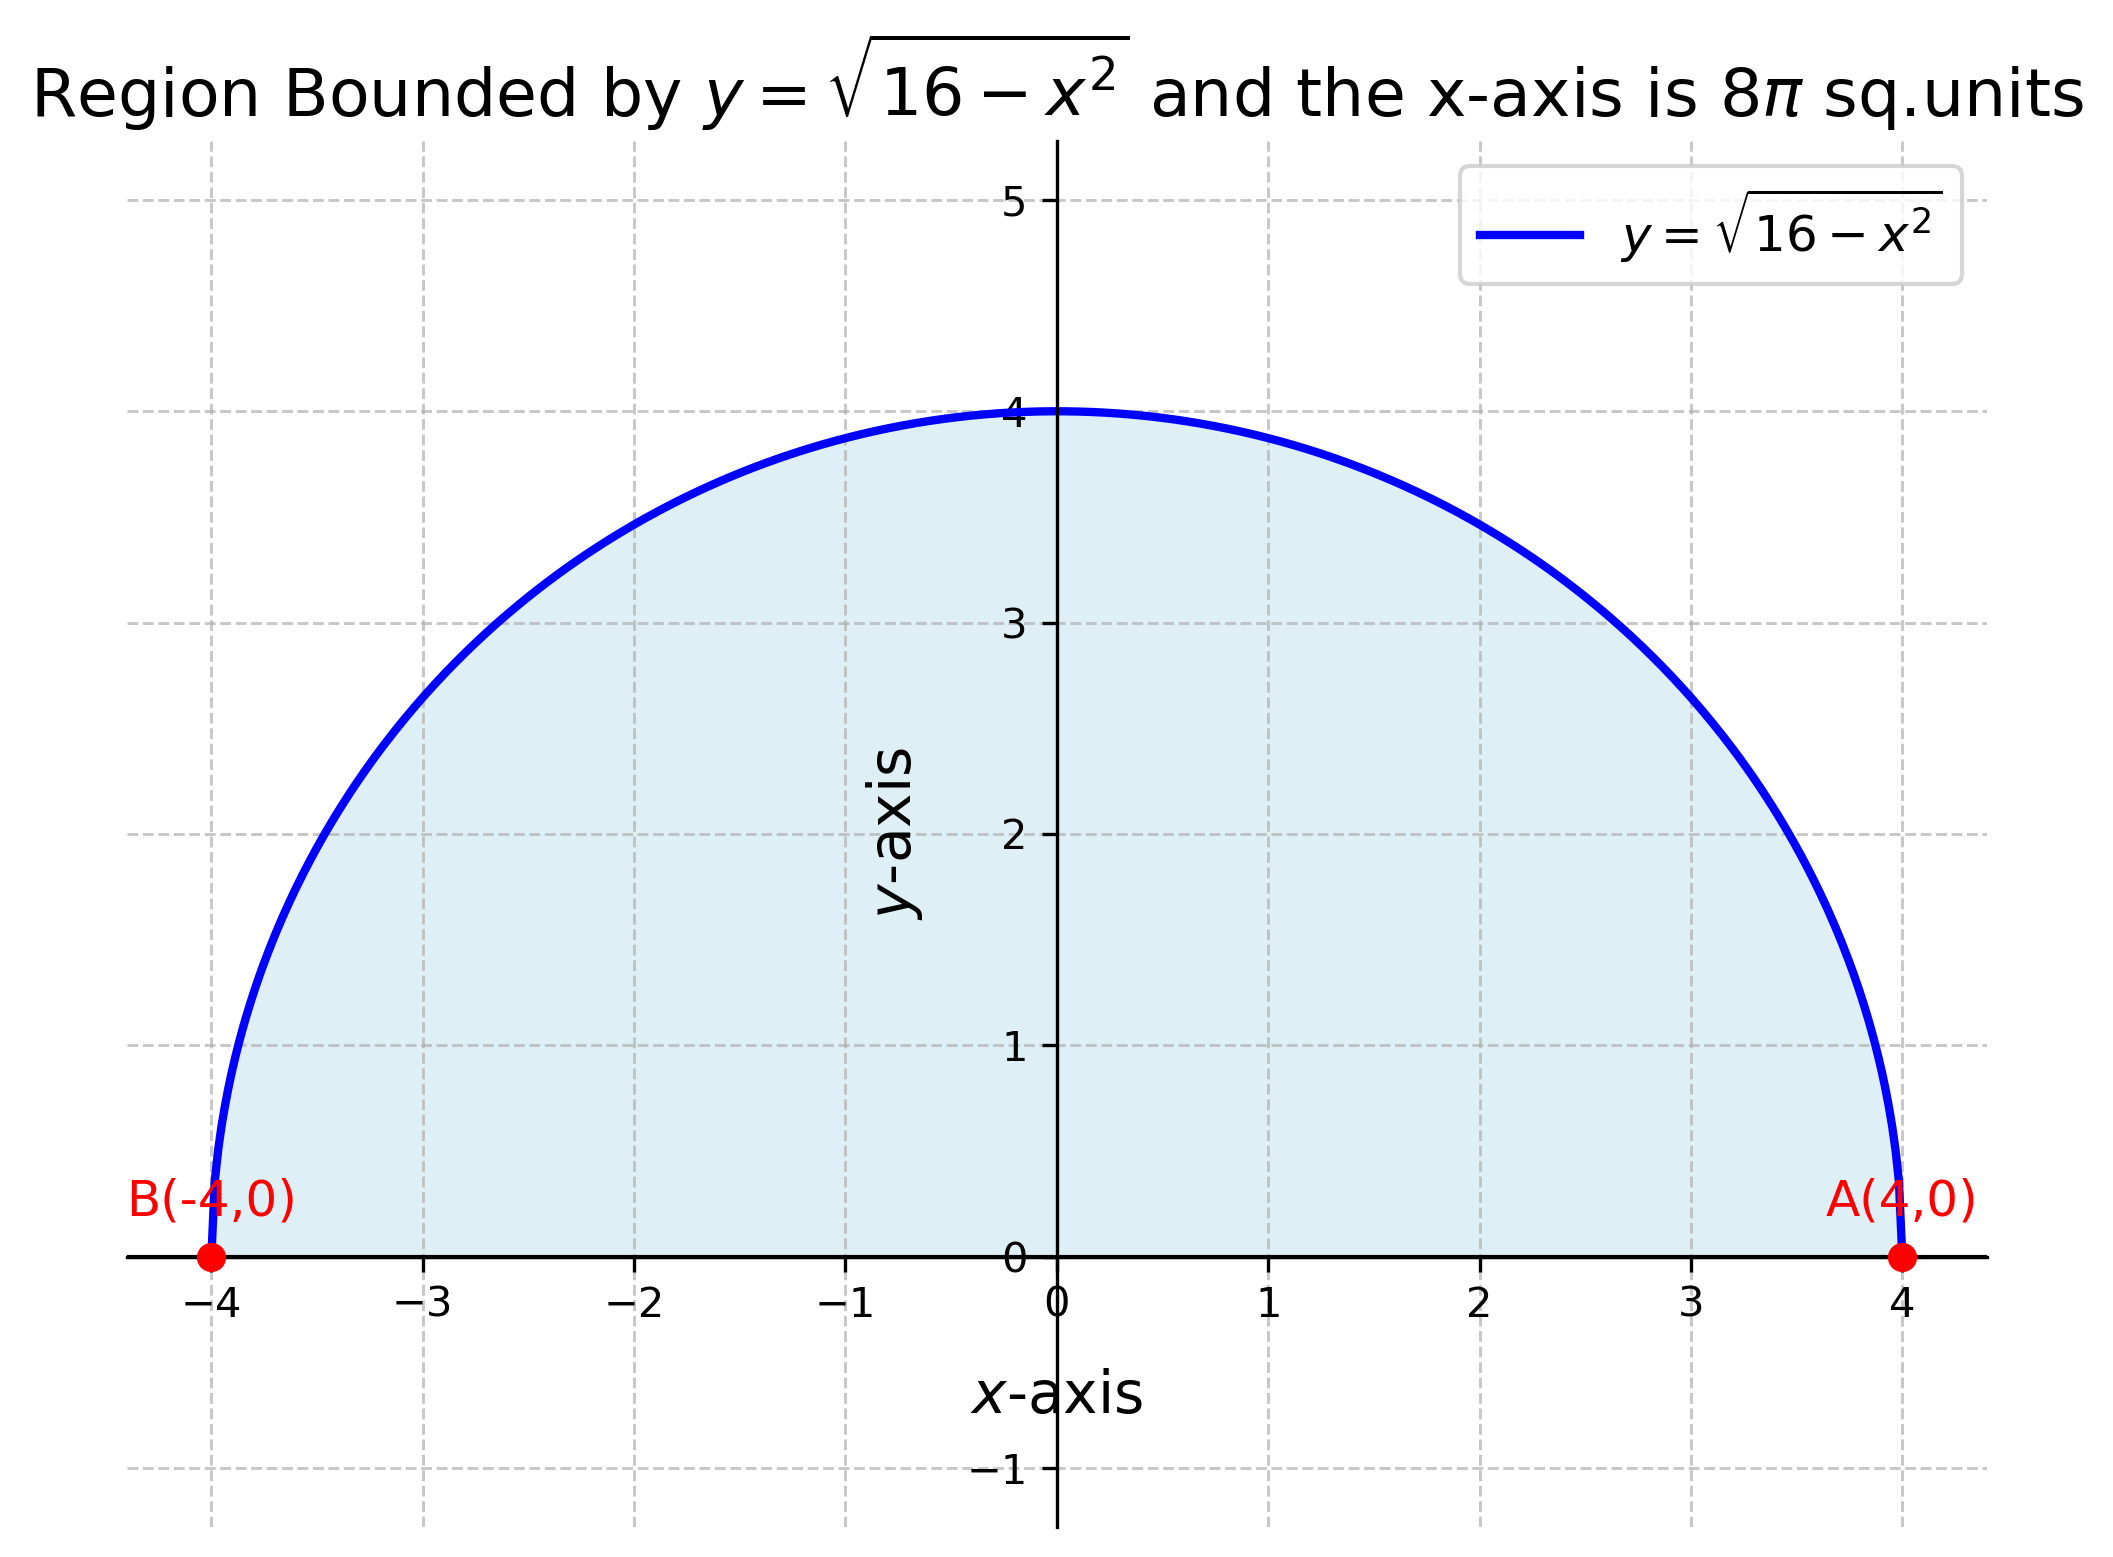
\includegraphics[scale=0.7]{figs/plot.png}
\label{Fig}
\end{figure}

%\frametitle{Introduction}
%\framesubtitle{Literature}
%%\begin{figure}[t!]
%%    \centering
%%    \begin{subfigure}[t]{0.4\columnwidth}
%%        \centering
%%        \includegraphics[width=\columnwidth]{point_source}
%%        \caption{Single point source}
%%\label{fig3:subfig1}        
%%    \end{subfigure}%
%%    ~ 
%%    \begin{subfigure}[t]{0.4\columnwidth}
%%        \centering
%%        \includegraphics[width=\columnwidth]{pointNoPowerDist_new}
%%        \caption{SNR profile}
%%\label{fig3:subfig2}
%%    \end{subfigure}
%%  %  \caption{Average SNR for a BPP. $N=16$}
%%    \label{fig3}
%%  \end{figure}
%
\end{frame}
%  
%
%
%%

\end{document}
